\documentclass{article} % For LaTeX2e
\usepackage{nips12submit_e,times}
%\documentstyle[nips12submit_09,times,art10]{article} % For LaTeX 2.09

% For figures
\usepackage{multirow}

\usepackage{graphicx} % more modern
%\usepackage{epsfig} % less modern
\usepackage{subfigure} 

% For citations
\usepackage{natbib}
\usepackage{subfigure}
% For algorithms
\usepackage{algorithm}
\usepackage{algorithmic}

% As of 2011, we use the hyperref package to produce hyperlinks in the
% resulting PDF.  If this breaks your system, please commend out the
% following usepackage line and replace \usepackage{icml2013} with
% \usepackage[nohyperref]{icml2013} above.
\usepackage{hyperref}
\nocite{*}

% Packages hyperref and algorithmic misbehave sometimes.  We can fix
% this with the following command.
\newcommand{\theHalgorithm}{\arabic{algorithm}}

% jovo added stuff
\newcommand{\iid}{\overset{iid}{\sim}}
\newcommand{\mbX}{\mathbf{X}}
\newcommand{\mbY}{\mathbf{Y}}
\newcommand{\Real}{\mathbb{R}}
\providecommand{\mh}[1]{\hat{#1}}
\providecommand{\mb}[1]{\boldsymbol{#1}}
\providecommand{\mc}[1]{\mathcal{#1}}
\newcommand{\from}{{\ensuremath{\colon}}}           % :
\usepackage{amsmath,amssymb,amsfonts}

\newcommand{\efoo}{\end{footnotesize}}
\newcommand{\bfoo}{\begin{footnotesize}}


% Employ the following version of the ``usepackage'' statement for
% submitting the draft version of the paper for review.  This will set
% the note in the first column to ``Under review.  Do not distribute.''

% Employ this version of the ``usepackage'' statement after the paper has
% been accepted, when creating the final version.  This will set the
% note in the first column to ``Proceedings of the...''
% \usepackage[accepted]{icml2013}

% jovo additions
\usepackage{color}
\newcommand{\jovo}[1]{{\color{magenta}{\it JoVo says: #1}}}
% \newcommand{\Real}{\mathbb{R}}
\usepackage{color}
\newcommand{\francy}[1]{{\color{blue}{\it Fra says: #1}}}
\newtheorem{theorem}{Theorem}%[section]
\newtheorem{lemma}[theorem]{Lemma}
\newtheorem{proposition}[theorem]{Proposition}
\newtheorem{corollary}[theorem]{Corollary}
\newtheorem{result}[theorem]{Result}
\newtheorem{definition}[theorem]{Def}


% The \icmltitle you define below is probably too long as a header.
% Therefore, a short form for the running title is supplied here:
\title{Multiresolution dictionary learning for conditional distributions}


%\nipsfinalcopy % Uncomment for camera-ready version

\begin{document}


\maketitle

\begin{abstract}
Nonparametric estimation of the conditional distribution of a response given high-dimensional features is a challenging problem.  In many settings it is important to allow not only the mean but also the variance and shape of the response density to change flexibly with features, which are massive-dimensional with a distribution concentrated near a lower-dimensional subspace or manifold.  We propose a  multiresolution model based on a novel stick-breaking prior placed on the dictionary weights.  The algorithm scales efficiently to massive numbers of features, and can be implemented efficiently with slice sampling.  State of the art predictive performance is demonstrated for toy examples and a real data application.
\end{abstract}


\section{Introduction}

Massive datasets are becoming a ubiquitous by-product of modern scientific and industrial applications. These data present statistical and computational challenges for machine learning because many previously developed approaches do not scale-up sufficiently.  Specifically, challenges arise because of the ultrahigh-dimensionality, and relatively low sample size (the ``large p, small n'' problem).  Parsimonious models for such big data assume that the density in the ambient dimension concentrates around a lower-dimensional (possibly nonlinear) subspace.  Indeed, a plethora of methodologies are emerging to estimate such lower-dimensional ``manifolds'' from high-dimensional data \cite{Manifold, Maggioni}.  

We are interested in using such lower-dimensional embeddings to obtain estimates of the conditional distribution of some target variable(s).  This \emph{conditional regression} setting arises in a number of important application areas, including neuroscience, genetics, and video processing.  For example, one might desire automated estimation of a predictive density for a continuous neurologic {\em phenotype} of interest, such as intelligence or a creativity score, on the basis of available data for a patient including neuroimaging.  The challenge is to estimate the probability density function of the phenotype {\em nonparametrically} based on an $\mathcal{O}(10^6)$ dimensional image of the subject's brain.  It is crucial to avoid parametric assumptions on the density, such as Gaussianity, while allowing the density to change flexibly with predictors.  Otherwise, one can obtain misleading predictions and poorly characterize predictive uncertainty.

There is a rich machine learning and statistical literature on conditional density estimation of a response $y \in \mathcal{Y}$ given a set of features (predictors) $x=(x_1, x_2, \ldots, x_p)\in \mathcal{X}$. Common approaches include hierarchical mixtures of experts \cite{mixtureexperts,jiang1999}, kernel methods \cite{fan1996,fanyim2004,holmes2010,fu2011}, Bayesian finite mixture models \cite{nott2012,tran2012,norets2012} and Bayesian nonparametrics 
\cite{griffin06, dunson2007, DunsonPark, chung2009, tokdar2010}.  

In general, there has been limited consideration of scaling to large $p$ settings, with the variational Bayes approach of \cite{tran2012} being a notable exception. For dimensionality reduction, Tran et al. follow a greedy variable selection algorithm.  Their approach does not scale to the sized applications we are interested in. For example, in a problem with $p=1,000$ and $n=500$, they reported a CPU time of 51.7 minutes for a single analysis.  We are interested in problems many orders of magnitude or more larger than this, and require a faster computing time while also accommodating flexible non-linear dimensionality reduction (variable selection is a limited sort of dimension reduction).  To our knowledge, there are no nonparametric density regression competitors to our approach, which maintain a characterization of uncertainty in estimating the conditional densities; rather, all sufficiently scalable algorithms provide point predictions and/or rely on restrictive assumptions such as linearity.  

In big data problems, scaling is often accomplished using divide-and-conquer techniques. Well known examples are classification and regression trees (CART) \cite{CART} and multivariate adaptive regression splines (MARS) \cite{MARS}. These algorithms fit surfaces to data by explicitly dividing the input space into a nested sequence of regions, and by fitting simple surfaces  within these regions. Though these methods are appealing in providing a simple, flexible and interpretable mechanism of dimension reduction, it is well known that single tree estimates commonly have high variance and poor performance.  There is a rich literature proposing improvements based on bagging \cite{Bagging}, boosting \cite{Boosting} and random forests \cite{RandomForest}. Though these algorithms can substantially improve mean square error performance, computation can be expensive and performance degrades as dimensionality $p$ increases.

In fact, a significant downside of divide-and-conquer algorithms is their poor scalability to high dimensional predictors. As the number of features increases, the problem of finding the best splitting attribute becomes intractable so that CART, MARS and multiple trees models cannot be efficiently applied. Also mixture of experts models become computationally demanding, since both mixture weights and dictionary densities are predictor dependent. In an attempt to make mixtures of experts more efficient, sparse extensions relying on different variable selection algorithms have been proposed \cite{SparseMoF}. However, performing variable selection in high dimensions is effectively intractable: algorithms need to efficiently search for the best subsets of predictors to include in weight and mean functions within a mixture model, an NP-hard problem.

 In order to efficiently deal with massive datasets, we propose a novel multiresolution approach which starts by learning a multiscale dictionary of densities, constructed as Gaussian within each set of a multiscale partition tree for the features. This tree is efficiently learned in a first stage using a fast and scalable graph partitioning algorithm applied to the high-dimensional features \cite{metis}.  Expressing the conditional densities $f(y|x)$ for each $x \in \mathcal{X}$ as a convex combination of coarse to fine scale dictionary densities, the learning problem in the second stage is how to estimate the corresponding multiresolution probability tree.  This is accomplished in a Bayesian manner using a novel multiresolution stick-breaking process, which allows the data to inform about the optimal bias-variance tradeoff; weighting coarse scale dictionary densities more highly decreases variance while adding to bias if the finer scale structure is needed.  This results in a model that allows borrowing information across different resolution levels and reaches a good compromise in terms of the bias-variance tradeoff. We show that the algorithm scales efficiently to massive numbers of features. 


\section{Setting} \label{section:setting}
Let $x \in \mathcal{X} \subseteq \Re^p$ be a $p$-dimensional Euclidean vector-valued predictor random variable.  Let $f(x)$ denote the marginal probability density of $x$.  We assume that $f(x)$ concentrates around a lower-dimensional, possibly nonlinear, subspace $\mc{M}$.  For example, $\mc{M}$ could be a union of affine subspaces, or a smooth compact Riemannian manifold.  

Let $y \in  \mathcal{Y} \subseteq \Re$ be a real-valued target variable. We further assume that the conditional distribution is a function of only the position $\mu$ of $x$ within the subspace $\mathcal{M}$, $f(y|x)=f(y|\mu)$. Let $x$ and $y$ be sampled from some true but unknown joint distribution. We would like to learn $f(y| x)$.  We assume that we obtain $n$ independently and identically sampled observations, $(x_i,y_i) $, for $i \in \{1,2,\ldots,n\}$.  Our proposed model introduced in \S \ref{section:model} is very general in accommodating an unknown density $f(y|x)$ which changes according to the location of $x$ in the lower-dimensional subspace.  However, for exposition and testing of the model, it is useful to consider a simple example in which $x$ lives on a smooth one-dimensional Riemannian submanifold embedded in $\Re^p$, and  $y$ is a univariate Gaussian random variable whose mean and variance vary with the location of $x$ along its geodesic.  

We can formalize this simple example model as follows. Consider  $$x_i \sim \mc{N}(\psi(\mu_i),\sigma^2 I),$$ where $\Psi =\{ \psi \from \mc{M} \to \Re^p\}$, $\mu_i \in \mc{M}$, $\sigma \in (0,\infty)$, $I$ is the $p\times p$ dimensional identity matrix.  Let $\mc{M}$ be a smooth compact Riemannian manifold, such as the swissroll or the S-manifold. For simplicity, let us assume that $\mc{M}$ is a curve. Let $\psi(\mu)= 1\mu$ with $1$ being a $p$-dimensional vector with all elements equal to $1$. Define the conditional $f(y|x)$ as a function of $\mu$, i.e. a mixture density with mixture weights depending on $\mu$.  We will show in \S \ref{section:simulation} that  our construction facilitates an estimate of the density of $y$.


\section{Model specification} \label{section:model}

Our approach proceeds in a two stage fashion as follows. We first learn a multiscale nonlinear partition tree of the feature data $\{ x_i \}_{i=1}^n$, recursively partitioning $\{x_i \}$ to obtain subsets that are increasingly homogeneous according to some metric.  The coarsest scale contains all of the data, the next finer scale contains two or more clusters of observations having relatively similar $x_i$ values, and so on  until our convergence criteria are met (for example, the available sample size is exhausted so that few observations fall within each fine scale leaf partition set).  Based on the multiscale partition, each value of $x$ has an associated path through the tree encoding the set membership at each scale.  Using the response data $y_i$ for all subjects $i$ in a given partition set, we estimate a dictionary density specific to that set and resolution level using Bayesian methods.  The conditional density is then expressed as a convex combination of these multiresolution dictionary densities, with a posterior distribution on the weights learned under a multiresolution stick-breaking process.

\begin{definition}\label{Def:tree} A tree decomposition of a $p$ dimensional space $\mathcal{X}$ is a collections of sets $\{\mathcal{X}^m_j\}_{j \in \mathcal{K}_m,m \in \mathcal{S}}$ satisfying:

(i) for every $m\in \mathcal{S}$, $\cup_{j=1}^{\mathcal{K}_j} \mathcal{X}^{m}_j=\mathcal{X}$ 

(ii) for every $j\not= j'$ and $m \in \mathcal{S}$, $\mathcal{X}_j^m \cap \mathcal{X}_{j'}^m=\emptyset$ 

(iii) for every $j$ and $m>1$ there is a $j'$ such that $\mathcal{X}^j_m \subset \mathcal{X}^{j'}_{m-1}$
\end{definition}

\noindent For simplicity we will focus on dyadic trees where each set is split into two subsets. Starting from generation one corresponding to the entire $\mathcal{X}$, denoted as $\mathcal{X}^1$, each set $\mathcal{X}^m_j$ is split into two mutually exclusive partition sets so that for a general partition level $m$ the partition will be given by $\mathcal{X}^{m}=\left(\mathcal{X}^{m}_1, \ldots, \mathcal{X}^{m}_{2^{m-1}}\right)$. Let us assume this process proceeds for $L$ levels and that all final leaves contain one element. Let $(m,s)$ be the node associated to the $s$th subset at resolution level $m$. Let $A_{m}(x) \in \{1, \ldots, 2^{m-1}\}$ be the location of predictor $x$ at level $m$, with $A_1(x)$ equal to 1 by definition.  The vector $A(x)=[A_1(x), \ldots, A_L(x)]$ encodes the path through the partition tree up to generation $L$ specific to predictor value $x$. Let $de(\ell,s)$ and $an(\ell,s)$ be respectively the set of descendants and ancestors of node $(\ell, s)$. \\

We characterize the conditional density $f(y|x)$ as a convex combination of multiscale dictionary densities.  At level one, the global parent density is denoted by $f_1$. For predictor value $x$, the dictionary density at generation $j$ is $f_{B_j(x)}$ with $B_j(x)=\{j,A_j(x)\}$, for $j=2,\ldots, k$. Then, $f(y|x)$ is defined as the convex combination of densities $\{f_{B_j(x)}\}_{j=1}^k$ with weights $\{\pi_{B_j(x)} \}_{j=1}^k$, i.e.
\begin{eqnarray}
f(y|x) = \sum_{j=1}^k \pi_{B_j(x)} f_{B_j(x)}(y),  \label{eq:base}
\end{eqnarray}
where $0 \le \pi_{B_j(x)}$ and $\sum_{j=1}^k \pi_{B_j(x)}=1$. 

Each $B(x)$ is a set encoding the path through the partition tree up to generation $k$ specific to predictor value $x$. According to model \eqref{eq:base}, one observation can lie in subsets located at different resolution levels. This is critical in achieving a good compromise between bias and variance through borrowing information across different resolution levels. Though the proposed approach is reminiscent of a mixture of experts model \cite{mixtureexperts}, the two approaches are quite different, since under \eqref{eq:base}, neither mixture weights nor dictionary densities directly depend on predictors. This allows our model to scale efficiently to high dimensional predictors.

Now let us examine the implications of model (\ref{eq:base}). For two predictor values $x$ and $x'$ located close together, it is expected that the paths will be similar, which leads to similar weights on the dictionary densities.  In the extreme case in which $x$ and $x'$ belong to the same leaf partition set, we have $B(x) = B(x')$ and the path through the tree will be the same.  Moreover, in this case, we will have $f(y|x)=f(y|x')$ so that up to $k$ levels of resolution the densities $f(y|x)$ and $f(y|x')$ are identical.  If the paths through the tree differ only in the final generation or two, the weights will typically be similar but the resulting conditional densities will not be identical. 

To derive mixture weights, a natural choice corresponds to a stick-breaking process \cite{stickbreaking}.  For each node $B_j(x_i)$ in the partition tree, define a stick length $V\{B_j(x_i)\} \sim \mbox{Beta}(1,\alpha)$.  The parameter $\alpha$ encodes the complexity of the model, with $\alpha=0$ corresponding to the case in which $f(y|x) = f(y)$.  We relate the weights in (\ref{eq:base}) to the stick-breaking random variables as follows: 
\begin{eqnarray*}
\pi_{B_j(x)} = V\left\{B_j(x)\right\} \prod_{B_h \in an\left\{B_j\right\}} \left[1 - V\left\{B_h(x)\right\}\right],
\end{eqnarray*}
with $V\{B_k(x)\}=1$ to ensure that $\sum_{j=1}^k \pi_{B_j}(x) = 1$.   We refer to this prior as a {\em multiresolution stick-breaking process}.   
\vskip 12pt


\section{Estimation}

The proposed approach is based on a two-stage algorithm where first the observations are allocated to different subsets in a tree fashion using an efficient partitioning algorithm and then, considering the partition as fixed, a multiresolution stick-breaking process is estimated. In practice, observations are partitioned applying metis \cite{metis}, a fast multiscale technique used for graph partitioning. 
% THE FOLLOWING MAKES NO SENSE
%Basically, the graph is obtained adding an edge between each pair of data points, i.e. $(y_i,y_j)$ with $i\not=j$, and assigning to any such edge the weight $w_{ij}=\exp\{-d(x_i,x_j)\}$ with $d(\cdot,\cdot)$ being some metric. 
Though more complicated densities can be considered, dictionary densities $f_{B_j}$ will be estimated by assuming a normal form, i.e. $f_{B_j}=\mc{N}(\mu_{B_j},\sigma_{B_j})$. In particular, densities corresponding to a particular partition set will be estimated considering only observations belonging to that partition set. To be specific, for estimating density $f_{B_j}(y)$, we use the data $\{ y_i: x_i \in \mathcal{X}^j_{A_j} \}$. We then conduct the analysis treating partition sets as fixed; this is critical for scalability to big $p$.  On the surface, conditioning on a single tree seems overly restrictive, but using a second stage multiresolution probability model for the weights over the tree leads to inferences that are robust to the tree estimate; almost as if the tree itself were randomized.

Parameters involved in the dictionary densities can be estimated using either frequentist or Bayesian methods. Bayesian methods are appealing since they can avoid singularities associated with traditional maximum likelihood inference, the prior has an appealing role as a regularizer, and we can characterize uncertainty in dictionary learning through the resulting posterior.
Hence, parameters involved in dictionary densities will be estimated through Bayesian methods and inference on stick breaking weights and dictionary density parameters will be carried out using the Gibbs sampler. For this purpose, introduce the latent variable $S_i \in \{1,\ldots,k\}$, for $i=1,\ldots,n$, denoting the multiscale level used by the $i$th subject.  Assuming data are normalized prior to analysis, we let $\mu \sim \mc{N}(0,I)$ and $\sigma=\mc{IG}(a,b)$ for the means and variances of the dictionary densities. Let $n_{B_j}$ be  the number of observations allocated to node $B_j$ . Each Gibbs sampler iteration can be summarized in the following steps.
\begin{enumerate}
\item Update $S_i$ by sampling from the multinomial full conditional with 
\[\mbox{Pr}( S_i = j\, |\, -) = \frac{ \pi_{B_j(x_i)}f_{B_j(x_i)}(y_i) }{ \sum_{h=1}^k \pi_{B_h(x_i)}f_{B_h(x_i)}(y_i) } \label{eq:prS}\]
\item Update stick-breaking random variable $V_{B_j(x_i)}$, for $j=1, \ldots, k$ and $i=1, \ldots, n$, from $\mbox{Beta}(\beta_p,\alpha_p)$ with $\beta_p=1+n_{B_j}$ and $\alpha_p=\alpha+\sum_{B_h(x_i) \in de\{B_j(x_i)\}} n_{B_h(x_i)}$.
\item Update $(\mu_{B_j(x_i)},\sigma_{B_j(x_i)})$ by sampling from
\[  \mu_{B_j} \sim \mc{N}\left(\bar{y}_{B_j} n_{B_j}/\sigma_{B_j},(1+n_{B_j}/\sigma_{B_j})^{-1}\right)\]
\[ \sigma_{B_j} \sim \mc{IG}\left(a_{\sigma},b+0.5\sum_{\{i: S_i=j,x_i \in B_j\}} \left(y_{i}-\mu_{B_j}\right)^2\right)\]
with $a_{\sigma}=a+n_{B_j}/2$, $\bar{y}_{B_j}$ being the average of the observation $\{y_i\}$ allocated to node $B_j$.

\end{enumerate}


\section{Simulation studies}\label{section:simulation}

In order to assess the predictive performance of the proposed model, different simulation scenarios were considered. Let $n$ be the number of observations, $y \in \Re$ the response variable and $x \in \Re^p$ a set of predictors. The Gibbs sampler was run considering $20,000$ as the maximum number of iterations with a burn-in of $1,000$. Gibbs sampler chains were stopped testing normality of normalized averages of functions of the Markov chain \cite{Chauveau98anautomated}. Parameters $(a,b)$ and $\alpha$ involved in the prior density of parameters $\sigma_{B_j}$s and $V_{B_j}$s were set respectively equal to $(3,1)$ and $1$.

In all simulation scenarios, predictors were assumed to belong to an $r$-dimensional space, either a lower dimensional plane or a non linear manifold, with $r<<p$. For each synthetic dataset, the proposed model was compared with CART and lasso in terms of mean squared error. For CART and Lasso standard Matlab packages were utilized. In order to fairly compare Lasso with the proposed model, a fast Lasso algorithm based on Lars was implemented and the regularization parameter was chosen based on  the AIC. 

\subsection{Illustrative Example}
First let us consider the simple toy example of \S \ref{section:setting}. We created an equally spaced grid of points $t_i=0, \ldots, 20$. Then, we let $\eta_i=\sin(t_i)$ and predictors be a linear function of $\eta_i$ plus Gaussian noise, i.e. $x_i=\eta_i + \epsilon_i$ with $\epsilon_i \sim N(0,0.1)$. The response was drawn from the following mixture of Gaussians
\begin{equation}
y_i \sim w_i \mathcal{N}(-2,1) + (1-w_i) \mathcal{N}(2,1) 
\end{equation}
with $w_i=|\eta_i|$. Our model was run considering different sample sizes. Figure \ref{plotDensity} shows the estimated density of two data points. These estimates were obtained by performing leave-one-out prediction for different number of observations in the training set. As the figure clearly shows our construction facilitates an estimate of the density $y$ that become closer to the true density as the number of observations in the training set increases.




\begin{figure}[h!]
\centering
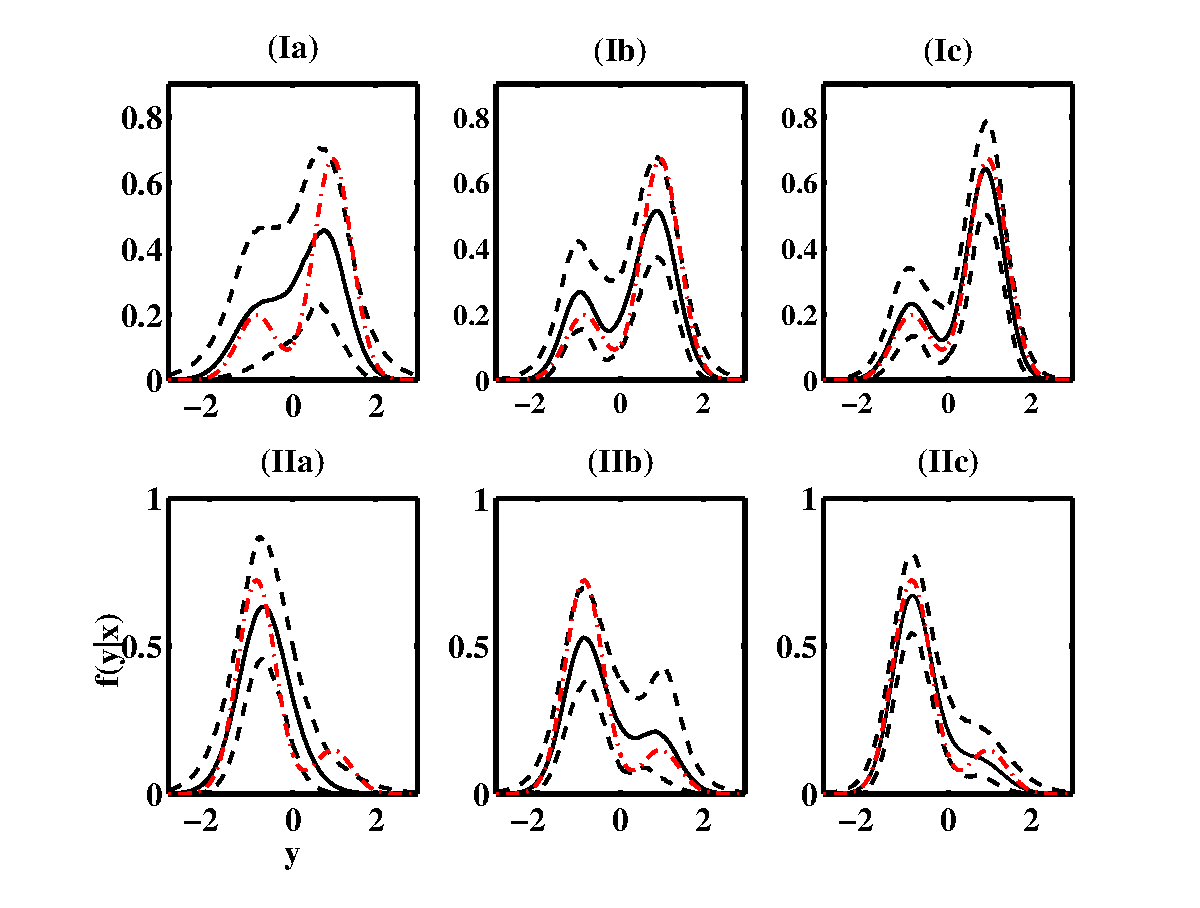
\includegraphics[width=0.8\linewidth]{densityestimate.eps}
% 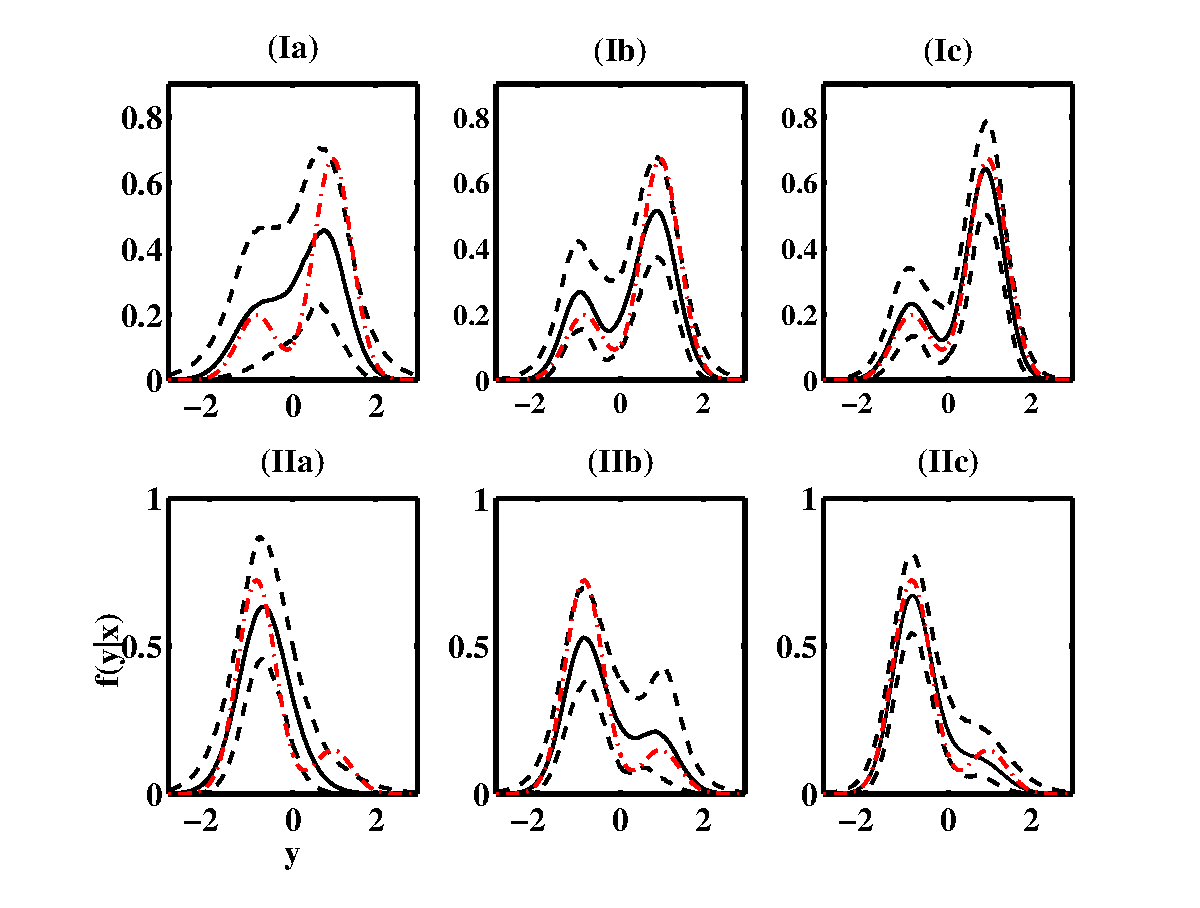
\includegraphics[width=90mm,height=80mm]{densityestimate.eps}
\caption{Illustrative example: Plot of true (red dashed-dotted line) and estimated ($50$th percentile: solid line, $2.5$th and $97.5$th percentiles: dashed lines) density for two data points $(I, II)$ considering different training set size (a:50, b:100, c:150). } \label{plotDensity}
\end{figure}

%% INSERT  For each resolution level, the new observation was allocated to the set with closer center. 

\subsection{Linear lower dimensional space} \label{section:linear}

In this section, the vector of predictors was assumed to lie close to a lower dimensional plane. In practice,  predictors were modeled through a factor model as follows 

\begin{equation} x_i=\Lambda \eta_i + \epsilon_i \end{equation} 

with $\epsilon_i \sim \mc{N}(0,\Sigma_0)$, $\Sigma_0=diag(\sigma_1, \ldots, \sigma_p)$, $\Lambda$ being a $p \times r$ matrix, $\eta_i \sim \mc{N}(0,I)$ and $r<<p$. In the first simulation scenario the response $y$ was assumed to be a function of the latent variable $\eta$ so that  the dependence between response and predictors was induced by the shared dependence on the latent factors. In practice, the pair $(y_i, x_i)$ was jointly sampled from a factor model. The loading matrix was derived as the product of a matrix with orthogonal columns and a diagonal matrix with positive elements on the diagonal, i.e. $\Lambda=\Gamma \Theta$. In particular, the columns of $\Gamma$ were uniformly sampled from the Stiefel manifold while the diagonal matrix of $\Theta$ were sampled from an inverse Gamma with shape and rate parameters $(1,4)$. In the second simulation scenario, $x$ was sampled from a factor model with sparse loading while $y$ was sampled from a normal with location and scale parameter $(1,1)$ if the first variable was positive, i.e. $x_1>0$, and from a normal with location and scale $(-1,1)$ otherwise. In this example, the non zero elements of the loading matrix were sampled from a normal with zero mean and standard deviation $3$. In all the examples, an inverse gamma prior with parameters $(1,4)$ were utilized for $\sigma_j$ with $j=1, \ldots, p$.

Table \ref{table:linear1} and \ref{table:linear2} show mean squared errors under the proposed approach, CART and lasso based on leave-one-out prediction. As shown in table \ref{table:linear1} and table \ref{table:linear2}, in almost all data scenario, our model is able to perform as well as or better than the model associated to the lowest mean squared error. In the first data scenario, given the linear relationship between response and predictors, Lasso performs better CART in almost all experiments. On the other hand, the non linear relationship between response and predictors assumed in the second data scenario results in better performance for CART. Table \ref{table:linear1} and figure \ref{Cpu} show the mean of CPU usage to predict a single point as a function of the number of features. In particular, CPU time is expressed in seconds and codes have been running on our workstation (Intel Core i7-2600K Quad-Core Processor memory 8192 MB).  Clearly, the proposed model scale substantially better than others to high dimensional predictors. 




\begin{table}[t]
\caption{Linear manifold example 1: Mean and standard deviations of squared errors under multiscale stick-breaking (MSB), CART and Lasso for sample size 50 and 100 for different simulation scenarios.}\label{table:linear1}
\vskip 0.15in
\begin{center}
\begin{small}
\begin{sc}
\begin{tabular}{lllcccccc}
\hline
&&&\multicolumn{3}{c}{$r=5$}&\multicolumn{3}{c}{$r=10$}\\
$p$&$n$& & msb&cart&lasso & msb&cart&lasso \\
\\
\multirow{3}{*}{$10^4$}&\multirow{3}{*}{50}&\bfoo mse\efoo&0.18&0.31&0.25&0.22&0.58&0.22\\
&&\bfoo std\efoo &0.32&0.30&0.42&0.24&0.54&0.30\\
&&\bfoo time\efoo &3&2&1&3&3&1\\

\\
\multirow{3}{*}{$10^4$}&\multirow{3}{*}{100}&\bfoo mse\efoo&0.18&0.27&0.26&0.20&0.41&0.52\\
&&\bfoo std\efoo & 0.26&0.42&0.46&0.23&0.46&0.78\\
&&\bfoo time\efoo &5&5& 2&5&5&1\\

\\
\multirow{3}{*}{$10^5$}&\multirow{3}{*}{50}&\bfoo mse\efoo&$0.35$&$0.45$&$0.89$&$0.16$&$0.33$&$0.20$\\
&&\bfoo std\efoo &$0.53$ &$0.77$&$1.04$&$0.21$&$0.46$&$0.31$\\
&&\bfoo time\efoo &$3$&$25$&$2$&$3$&$27$&$2$\\
\\
\multirow{3}{*}{$10^5$}&\multirow{3}{*}{100}&\bfoo mse\efoo&$0.43$&$0.88$&$0.52$&$0.17$&$0.50$&$0.31$\\
&&\bfoo std\efoo &$0.59$ &$1.29$&$0.70$&$0.24$ &$0.75$&$0.49$\\
&&\bfoo time\efoo &$7$&$50$&$5$&$7$&$51$&$5$\\
\\
\multirow{3}{*}{$50^5$}&\multirow{3}{*}{50}&\bfoo mse\efoo&0.11&0.16&0.15&0.83&2.26&0.92\\
&&\bfoo std\efoo&$0.15$ &0.24&0.19&1.01&2.60&3.69\\
&&\bfoo time\efoo &5&90&11&5&121&10\\


\\
\multirow{3}{*}{$50^5$}&\multirow{3}{*}{100}&\bfoo mse\efoo&0.003&0.17&0.08&0.13&1.37&1.06\\
&&\bfoo std\efoo &0.16&0.23&0.13&1.12&1.81&1.50\\
&&\bfoo time\efoo &10&214&43&8&227&42\\

\\
\multirow{3}{*}{$70^5$}&\multirow{3}{*}{50}&\bfoo mse\efoo&1.70&1.48&1.47&0.66&1.65&1.07\\
&&\bfoo std\efoo &2.18&2.47&1.63&0.87&1.49&0.95\\
&&\bfoo time\efoo &6&121&12&7&151&13\\

\\
\multirow{3}{*}{$70^5$}&\multirow{3}{*}{100}&\bfoo mse\efoo&0.69&1.36&0.82&0.78&1.52&1.43\\
&&\bfoo std\efoo &0.94&1.47&1.28&1.03&1.34&2.11\\
&&\bfoo time\efoo &13&321&41&12&325&44\\

 \hline
\end{tabular}
\end{sc}
\end{small}
\end{center}
\vskip -0.1in
\end{table}


\begin{table}[t]
\caption{Linear manifold example 2: Mean and standard deviations of squared errors under multiscale stick-breaking (MSB), CART and Lasso for sample size 50 and 100}\label{table:linear2}
\vskip 0.15in
\begin{center}
\begin{small}
\begin{sc}
\begin{tabular}{lllcccccc}
\hline
&&&\multicolumn{3}{c}{$r=2$}&\multicolumn{3}{c}{$r=5$}\\
$p$&$n$& & msb&cart&lasso & msb&cart&lasso \\

%\multirow{3}{*}{$10^5$}&\multirow{3}{*}{100}&\bfoo mse\efoo&0.63 &0.83&0.93&0.71&0.98&0.86\\
%&&\bfoo std\efoo &0.81&0.94&1.02&0.69 &1.04&1.55\\
%&&\bfoo time\efoo &9.45 &46.15& 4.55&8.05&47.65&5.15\\
%
%\\
%\multirow{3}{*}{$20^5$}&\multirow{3}{*}{100}&\bfoo mse\efoo&0.89&0.74&1.08&0.95 &&1.15\\
%&&\bfoo std\efoo &1.50 &1.02&1.97&1.20&&1.13\\
%&&\bfoo time\efoo &7.96&102.12&8.95& 10.70&&8.75\\
%
%\\
%\multirow{3}{*}{$50^5$}&\multirow{3}{*}{100}&\bfoo mse\efoo &0.83 &&0.94\\
%&&\bfoo std\efoo &1.08&koala&1.10\\
%&&\bfoo time\efoo &9.27&&23.54\\
\\

\multirow{2}{*}{$10^4$}&\multirow{2}{*}{100}&\bfoo mse\efoo&1.54 &1.78&2.37&0.84&1.25&1.62\\
&&\bfoo std\efoo &1.70&1.72&0.89&1.38&1.35&1.47\\


\\
\multirow{2}{*}{$50^4$}&\multirow{2}{*}{100}&\bfoo mse\efoo&0.76&0.97&1.77&0.88&1.53&1.43\\
&&\bfoo std\efoo &1.04&1.21&3.13&1.00&1.59&2.73\\

\\

\multirow{2}{*}{$10^5$}&\multirow{2}{*}{100}&\bfoo mse\efoo&0.77 &1.01&1.61&0.67&0.46&0.97\\
&&\bfoo std\efoo &0.94&1.13&1.85&0.82&0.61&1.16\\
%&&\bfoo time\efoo &7.69 &46.14&4.51&9.89&41.68&4.38\\
\\

\multirow{2}{*}{$20^5$}&\multirow{2}{*}{100}&\bfoo mse\efoo&0.86&0.90&1.41&0.74&1.09&0.78\\
&&\bfoo std\efoo &1.30&1.35&1.41&0.95&1.98&0.95\\
%&&\bfoo time\efoo &8.94&& 8.86 & 9.09&&17.17\\
%
%\\
%\multirow{2}{*}{$30^5$}&\multirow{2}{*}{100}&\bfoo mse\efoo&0.78&&1.32&&&\\
%&&\bfoo std\efoo &0.60&&1.27&&&\\
\hline
\end{tabular}
\end{sc}
\end{small}
\end{center}
\vskip -0.1in
\end{table}

\subsection{Non-Linear lower dimensional space}

In this section predictors were assumed to lie close to a lower dimensional non-linear manifold. In the first simulation study, predictors and response were jointly sampled from an $N$ components mixture of factor analyzers (see equation \ref{MFA}) so that the vector of predictors and response were assumed to lie close to $N$ lower dimensional planes. For each mixture components, the loading matrix and variances were sampled as in the first simulation scenario in \S \ref{section:linear}, while mixture weights were sampled from a Dirichlet distribution with parameter $\alpha_j=1$ for $j=1, \ldots, N$. The number of latent factors was considered to be increasing in the number of components, in practice we let the $h$th mixture component be modeled through $h$ factors. In the other simulation scenarios predictors were assumed to lie close to the Swissroll and the S-manifold (see figure \ref{manifold:nonlinear}), all two dimensional manifold embedded in $\Re^p$ while the response was sampled from a normal with mean equal to one of the coordinates of the manifold and standard deviation one.

As in \S \ref{section:linear}, the proposed model was compared in terms of computational time and predictive performance with lasso and Cart. Table \ref{table:mfa} and \ref{table:swiss}  show computational time and mean squared errors based on leave-one-out predictions considering each of the three simulation scenario.  In particular, table \ref{table:mfa} shows the results associated to the data drawn from the mixture of factor analyzers for different number of components. In this example, given the linear relationship between predictors and response, Lasso performs better than CART. Lasso is also much more efficient than CART and performs similarly to our model for moderately high dimensional features. However, as shown in table \ref{table:mfa}, as the sample size increases the computational time associated to Lasso dramatically increases compared to our model (see $p=300,000$ for $n=100, 200, 300$). Table \ref{table:swiss} also shows that our model is associated to better predictive performance and CPU time on massive dimensional predictors.


\begin{table}[t]
\caption{Non-linear manifold - MFA: Mean and standard deviations of squared errors under multiscale stick-breaking (MSB), CART and Lasso for sample size 50 and 100 for different simulations sampled from a mixture of factor analyzers}\label{table:mfa}
\vskip 0.15in
\begin{center}
\begin{small}
\begin{sc}
\begin{tabular}{lllcccccc}
\hline
&&&\multicolumn{3}{c}{$N=10$}&\multicolumn{3}{c}{$N=5$}\\
$p$&$n$& sim& msb&cart&lasso & msb&cart&lasso\\
\\
\multirow{3}{*}{$50^3$}&\multirow{3}{*}{100}&mse&0.23&0.42&0.36&0.17&0.43&0.22\\
&&std & 0.34 &0.59&0.43&0.18&0.69&0.23\\
&&time &5&24 & 3&7&27&3\\

\\
\multirow{3}{*}{$50^3$}&\multirow{3}{*}{200}&mse&0.23 &0.42 &0.27&0.17&0.22&0.20\\
&&std & 0.33& 0.56&0.23&0.19&0.38&0.25\\
&&time & 10 &51&8&12&56&7\\

\\
\multirow{3}{*}{$10^4$}&\multirow{3}{*}{100}&mse&0.67&1.35&1.32&0.15&0.17&0.22\\
&&std & 1.04&2.26&1.36&0.23&0.19&0.23\\
&&time &9&47&6&6&44&5\\

\\
\multirow{3}{*}{$10^4$}&\multirow{3}{*}{200}&mse&0.64&1.37&0.85&0.15&0.26&0.15\\
&&std &0.95 &1.77&1.29&0.24&0.42&0.24\\
&&time &15&99&15&11&89&15\\
\\
\multirow{3}{*}{$30^4$}&\multirow{3}{*}{100}&mse& 0.26&0.39&0.31&0.63&1.40&1.01\\
&&std &0.39&0.51&0.52&0.80 &1.24& 1.46 \\
&&time &9.28&125&18&9 &145& 17\\
\\
\multirow{3}{*}{$30^4$}&\multirow{3}{*}{200}&mse&0.25&0.47&0.26&0.63&1.17&0.92\\
&&std &0.36&0.88&0.43 & 0.80&2.11&1.04 \\
&&time &15&262&40&13&283&43\\


\\
\multirow{3}{*}{$30^4$}&\multirow{3}{*}{300}&mse&0.25&0.30&0.30&0.62&1.42&0.70\\
&&std &0.36&0.41&0.48&0.89&1.85&0.94\\
&&time &15&463&73&16&465&89\\

\hline
\end{tabular}
\end{sc}
\end{small}
\end{center}
\vskip -0.1in
\end{table}


\begin{figure}
\centering
\begin{tabular}{cc}
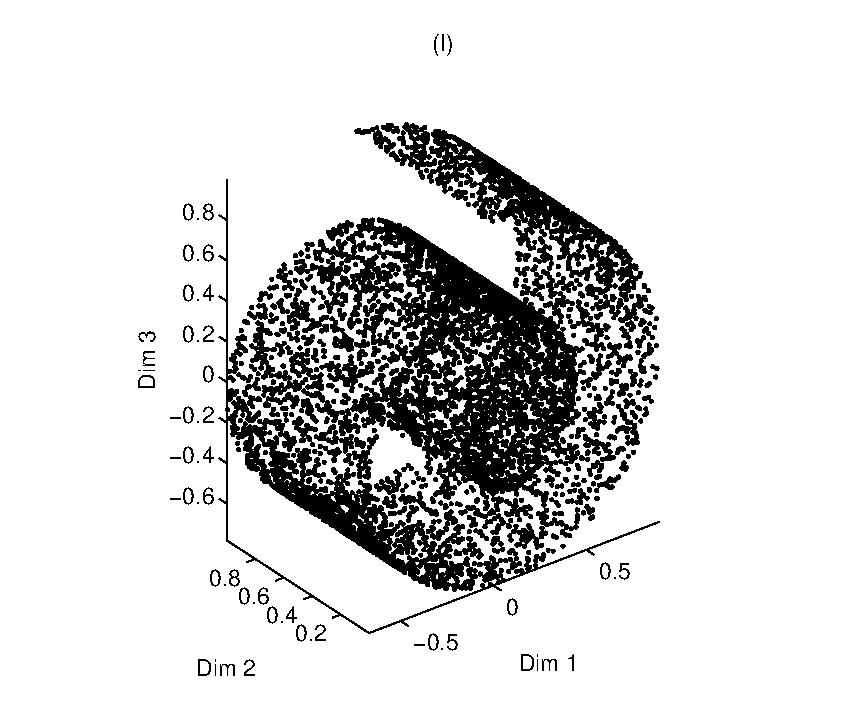
\includegraphics[width=90mm,height=60mm]{Swissroll.eps} & 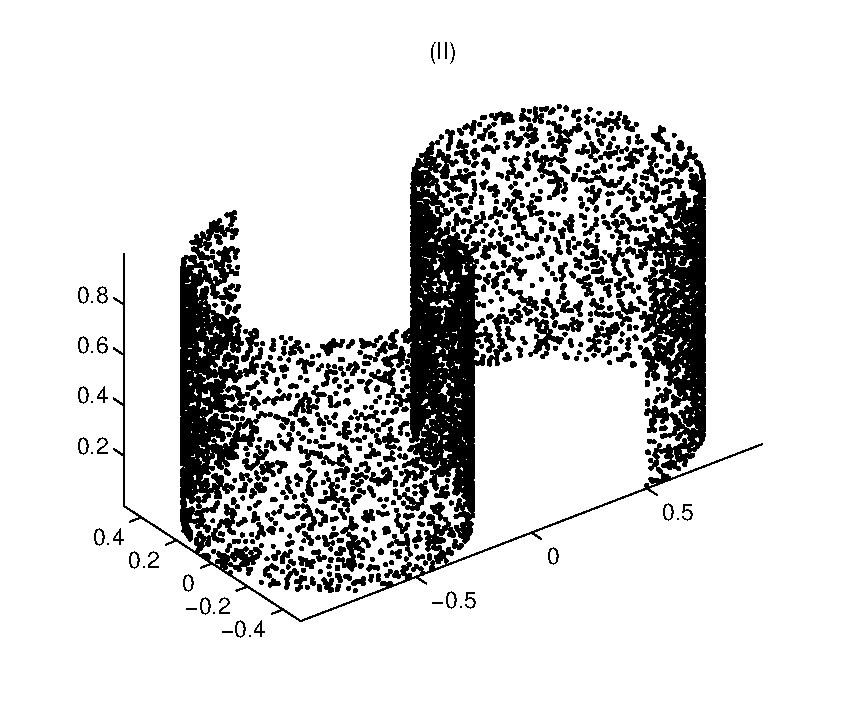
\includegraphics[width=60mm,height=60mm]{SManifold.eps}
\end{tabular}
\caption{Non-linear manifolds: Swissroll (I) and S-Manifold (II) embedded in $\mathcal{R}^3$} \label{manifold:nonlinear}
\end{figure}


\begin{table}[t]
\caption{Non-linear manifold - Swissroll and S-Manifold: Mean and standard deviations of squared errors under multiscale stick-breaking (MSB), CART and Lasso for sample size 50 and 100 for different simulation scenarios.}\label{table:swiss}
\vskip 0.15in
\begin{center}
\begin{small}
\begin{sc}
\begin{tabular}{lllcccccc}
\hline
&&&\multicolumn{3}{c}{Swissroll}&\multicolumn{3}{c}{S-Manifold}\\

$p$&$n$& & msb&cart& lasso & msb&cart& lasso\\
\\
\multirow{3}{*}{$10^4$}&\multirow{3}{*}{100}&mse &$0.25$&$0.46$&$0.38$\\
&&std & $0.24$ & $0.53$&$0.40$\\
&&time & 5& $5$&$1$ \\

\\
\multirow{3}{*}{$10^5$}&\multirow{3}{*}{50}&mse &$0.24$&$0.44$&$0.25$\\
&&std & $0.24$ & $0.42$&$0.29$\\
&&time & 3 & $22$&$2$ \\

\\
\multirow{3}{*}{$10^5$}&\multirow{3}{*}{100}&mse &$0.24$ & $0.43$&$0.17$\\
&&std & $0.26$&$0.55$&$0.22$\\
&&time&$6$&$48$&$7$\\
\\

\multirow{3}{*}{$20^5$}&\multirow{3}{*}{50}&mse &$0.24$&$0.67$&$0.29$\\
&&std & $0.23$ & $0.50$& $0.29$\\
&&time & 4& $38$& $5$ \\
\\
\multirow{3}{*}{$20^5$}&\multirow{3}{*}{100}&mse &$0.25$&$0.78$&$0.33$\\
&&std & $0.26$ & $0.74$&$0.36$\\
&&time &6 &$96$&$13$ \\
\\

\multirow{3}{*}{$50^5$}&\multirow{3}{*}{50}&mse &$0.17$&$0.47$&$0.23$\\
&&std & $0.23$ & $0.43$&$0.22$\\
&&time &$5$ &$126$&$10$ \\

\\
\multirow{3}{*}{$50^5$}&\multirow{3}{*}{100}&mse &$0.17$&$0.33$&$0.19$\\
&&std & $0.21$ &$0.46$ &$0.23$\\
&&time &$11$ &$230$&$25$\\



\hline
\end{tabular}
\end{sc}
\end{small}
\end{center}
\vskip -0.1in
\end{table}








\section{Real application}

We assessed the predictive performance of the proposed method on two very different neuroimaging datasets. First, we consider a structural connectome dataset collected at the Mind Research Network.  Data were collected as described in Jung et al. \cite{Jung2010}.
% ,and structural connectomes were estimated using the Magnetic Resonance Connectome Automated Pipeline \cite{MRCAP}.  
% Each of the $108$ children underwent both multimodal imaging and a battery of cognitive assessments.  
We investigated the extent to which we could predict creative (as measured via the Composite Creativity Index \cite{Arden2010}).   For each subject, we estimate a $70$ vertex undirected weighted brain-graph using the Magnetic Resonance Connectome Automated Pipeline \cite{MRCAP11} from diffusion tensor imaging data \cite{Mori2006}. We therefore let each $x_i \in \Re^p$ correspond to logarithm of each weighted edge; because our graphs are undirected and lack self-loops, we have a total of $\binom{70}{2}=2,415$ potential weighted edges.
The vector of covariates consists in the natural logarithm of the total number of connections between all pairs of cortical regions, i.e. $p=2,415$. 

The second dataset comes from a resting-state functional magnetic resonance experiment as part of the Autism Brain Imaging Data Exchange \cite{Autism}.  We selected the Yale Child Study Center for analysis.  Each brain-image was processed using the Configurable Pipepline for Analysis of Connectomes \cite{cpac}. For each subject we computed a measure of normalized power at each voxel called fALFF \cite{Zou2008}.  fALFF is a highly nonlinear transformation of the time-series data, previously demonstrated to be a reliable property of such data.  To ensure the existence of nonlinear signal relating these predictors, we let $y_i$ correspond to an estimate of overall head motion in the scanner, called mean framewise displacement (FD) computed as described in Power et al. \cite{power}.  We utilized a gray matter mask to consider only the voxels with high probability of being gray matter. Thus, for each of $56$ subjects, we let $x_i \in \Re^{300,000}$ be the fALFF of all gray matter voxels.

% Our interest was predicting the head motion measurement based on $3$D brain images involving about one million of pixels. These $3$D matrices were vectorized and considered as predictors in our model. In order to reduce the dimensionality of the predictor space the data was re-processed using a brain mask and a vector of about $300,000$ predictors  was obtained.

For the analysis, all variables were normalized by subtracting the mean and dividing by the standard deviation. The same prior specification and Gibbs sampler as in \S 5 was  utilized. Table \ref{real} shows mean and variance squared error based on leave-one-out predictions. Variable $t_{T}$ is the amount of time necessary to obtain predictions for all subjects, while variables $t_M$ and $t_V$ are respectively the mean and the standard deviation of amount of time necessary to obtain one point predictions.

For the first data example, we compared our approach (multiresolution stick-breaking; MSB) to CART, lasso and random forests. 
Table \ref{real} shows that MSB outperforms all the competitors in terms of mean square error; this is in addition to yielding an estimate of the entire conditional density for each $y_i$.  It is also significantly faster that random forests, the next closest competitor, and faster than lasso.  For this relatively low-dimensional example, CART is reasonably fast.  

 % random forest in terms of mean squared error, and is associated to a much lower CPU time. This real data application does not involve a huge number of predictors so that computationally our model performs almost as well as lasso and CART. However, as  shown in section 5, our model can scale substantially better than all other models to huge number of features. \\
 
 For the second data application, given the huge dimensionality of the predictor space, we were unable to get either CART or random forest to run to completion, yielding memory faults on our workstation (Intel Core i7-2600K Quad-Core Processor memory 8192 MB).  We thus only compare performance to lasso.  As in the previous example, MSB outperforms lasso in terms of predictive accuracy measured via mean-squared error, and significantly outperforms lasso in terms of computational time.  
 % and the poor scalability of CART and random forest, the comparison was made only with lasso. As shown in table \ref{real}, our approach is more efficient and accurate than lasso in predicting the response variable. 
Figure \ref{fig:real} shows the plot of CPU time used to predict each one of the $56$ subjects involved in the experiment. The time needed to compute quantities utilized in all subject predictions was divided equally across subjects. Clearly, our approach is able to improve the computational time by up to five orders of magnitude. 


\begin{table}[t]
\caption{Real Data: Mean and standard deviations of squared error under multiscale stick-breaking (MSB), CART, Lasso and random forest (RF).}\label{real}
\vskip 0.15in
\begin{center}
\begin{small}
\begin{sc}
\begin{tabular}{llccccccc}
\hline
data  &model&mse&$t_{T}$ & $t_{M}$ & $t_{V}$\\
\hline
(1)&msb &$0.56$ & $100$ & $1.1$& $0.02$\\
 & cart & $1.10$ & $87$ & $0.9$ &$0.01$\\
& lasso & $0.63$  & $200$ & $2.8$ & $0.17$\\
& rf & $0.57$ &  $7,817$ & $78.2$ & $0.59$\\
\\
  (2)&msb &$0.76$ & $690$ & $20.98$& $2.31$\\
 & lasso & $1.02$  & $5,836$ & $96.18$ & $9.66$\\
\hline
\end{tabular}
\end{sc}
\end{small}
\end{center}
\vskip -0.1in
\end{table}


\nocite{langley00}



\begin{figure}[h!]
\centering
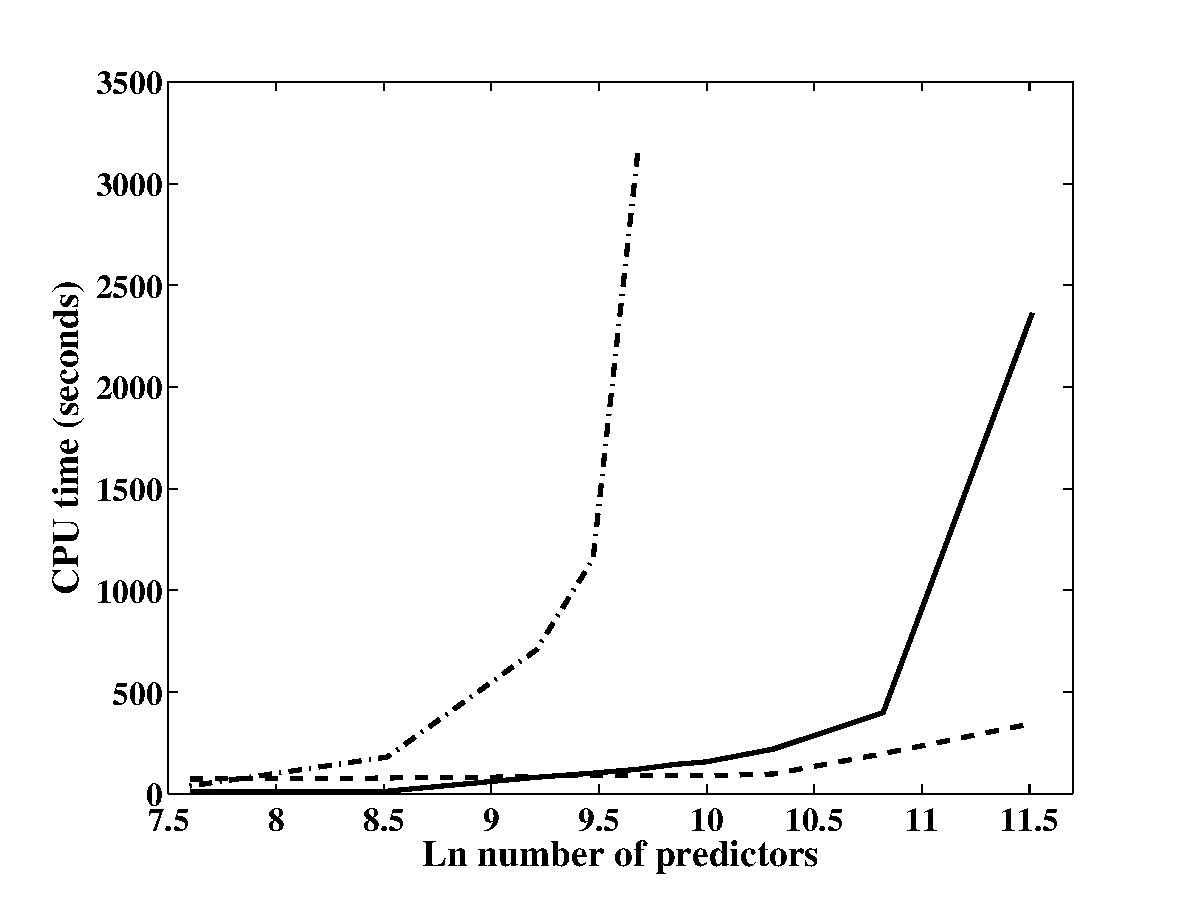
\includegraphics[width=0.8\linewidth]{Cpu.eps}
% 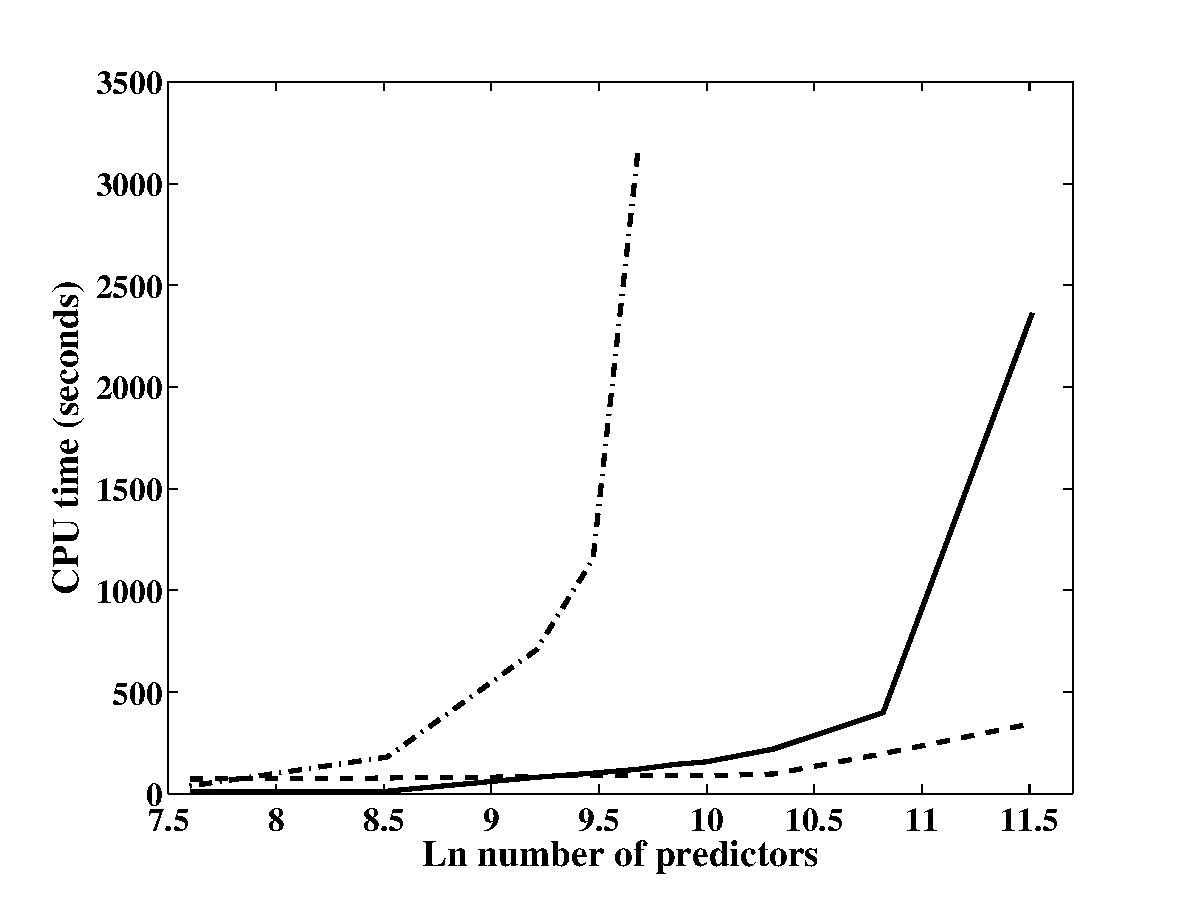
\includegraphics[width=80mm,height=45mm]{Cpu.eps}
\caption{Elapsed CPU time (in seconds) for leave-one-out prediction based on $100$ observations for MSB (dash), lasso (solid) and CART (dot-dash) for different number of predictors in log-scale.} \label{Cpu}
\end{figure}

\begin{figure}[h!]
\centering
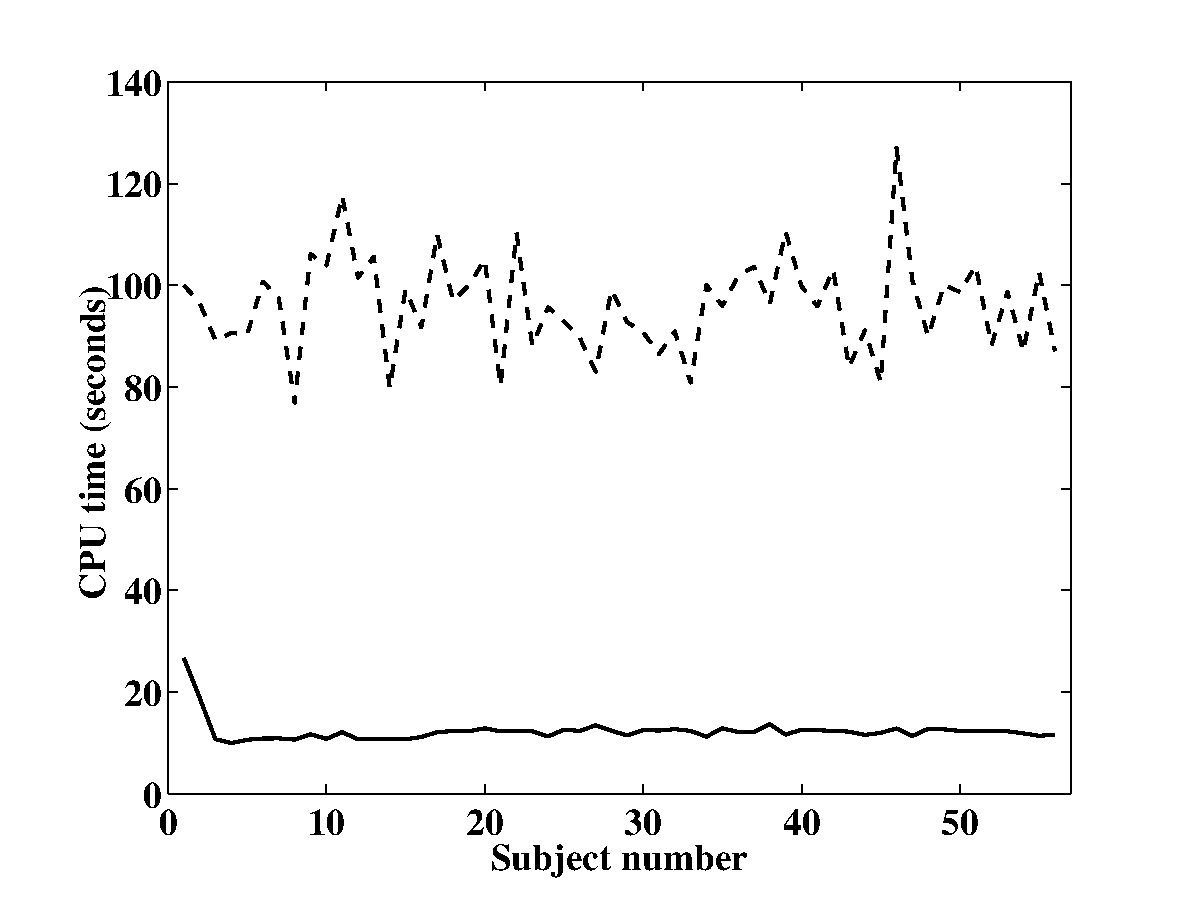
\includegraphics[width=1.0\linewidth]{Time_real2.eps}
% 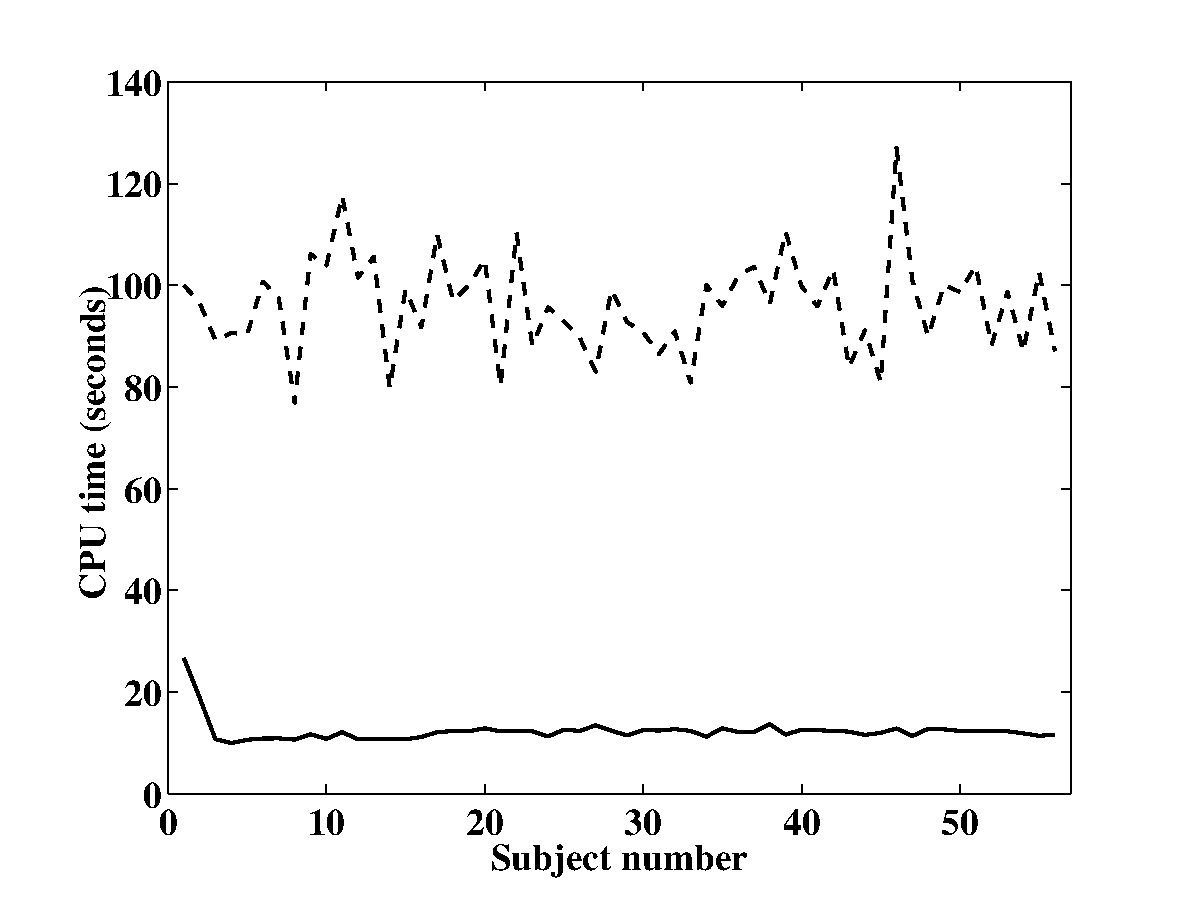
\includegraphics[width=80mm,height=40mm]{Time_real2.eps}
\caption{Plot of CPU time used to predict each one of the $56$ measurement involved in experiment (2) under MSB (solid) and lasso (dash).} \label{fig:real}
\end{figure}

\section{Conclusion}
We have proposed a new model which should lead to substantially improved predictive and computational performance to learn the density of a target variable given a high dimensional vector of predictors. As shown the proposed two stage approach can scale substantially better than other existing algorithms to massive number of features. We have focused on Bayesian MCMC-based methods, but there are numerous interesting directions for ongoing research. Moreover, in addition to better predictive and computational performance, our methods easily extend to parallelized and distributed systems, which we will also explore in future work.


\end{document}
